\chapter{Analysis}

The first objective is to ascertain the algorithm used by the Freestyle Libre reader to arrive at calibrated values, as well as to investigate if this can be improved.

The processed data\footnote{Herein, processed data refers to data collected from the reader, and raw data likewise refers to data directly extracted from the sensor.} - provided by \$history - is distinctly different from the raw  data. As discussed above, the sensor collects data every minute and provides some of this high definition data when scanned. As Figure~\ref{fig:graph3} shows, the processed data is consistently spaced 15 minutes apart, showing that it isn’t merely storage for the raw data. This is emphasized by Figure~\ref{fig:graph3}, which shows that the two datasets clearly don’t match. Most likely, the processed data is a processed version of the 15 minute raw data. Alternatively, the reader may process all raw data, including the high definition, then discard the extras to save space. Both have the same result; all data stored on the reader has been processed.

\begin{figure}[ht]
\centering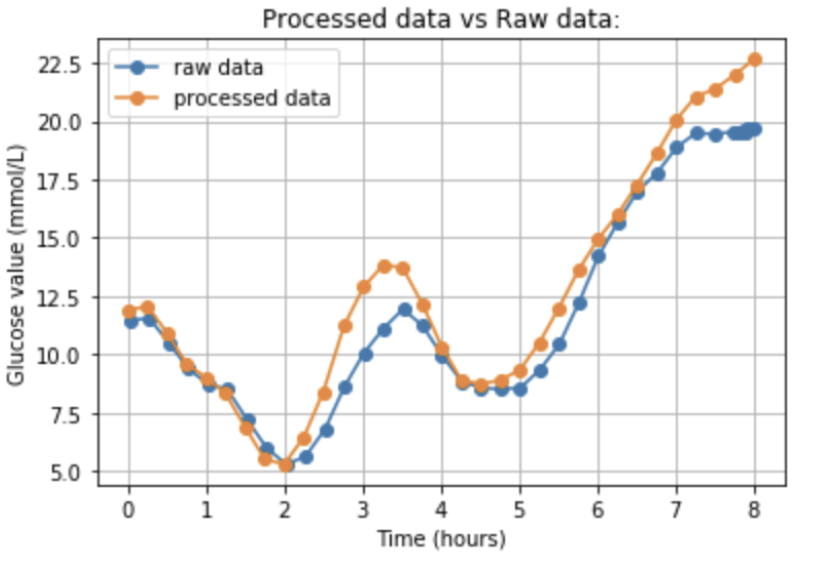
\includegraphics[width=1.0\linewidth]{images/graph3.png}
\caption{Graph of processed(reader) and raw(sensor) data.}
\label{fig:graph3}
\end{figure}

The data displayed on demand with each scan is intended to estimate the current blood glucose level - let's call this read-time data (alternatively manual data, since it is affected by the manual scanning of the sensor). It is clearly formulated from either or both of the processed and raw data. Surprisingly, the processing is not the same as for the other processed data. As seen in Figure~\ref{fig:graph4}, the manually pulled values heavily deviate from the other processed data. The most obvious reason for this would be an attempt to make up for the time lag between interstitial fluid and blood glucose. On the other hand, this could also be part of the initial formula for the processed data, which Figure~\ref{fig:graph3} would appear to support. Another option is that, if the processed data is calculated solely off of 15 minute data, the manual data is different because it also factors in the higher definition one minute data. 

\begin{figure}[ht]
\centering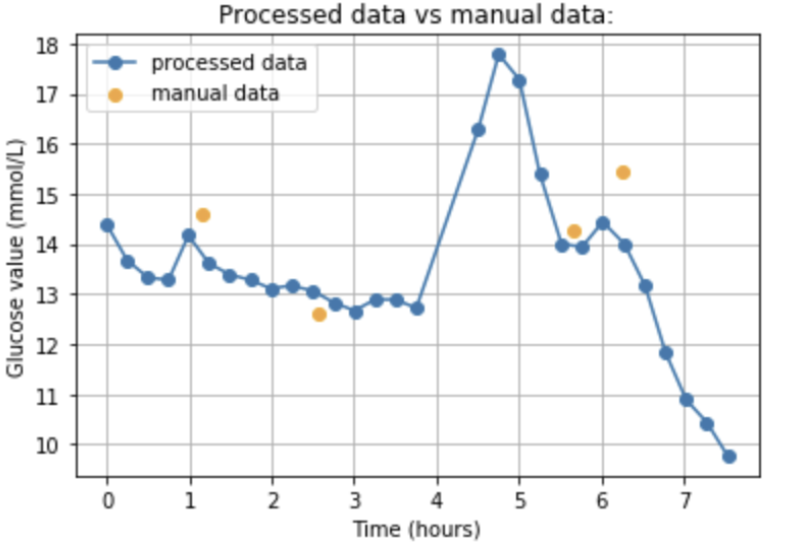
\includegraphics[width=1.0\linewidth]{images/graph4.png}
\caption{Graph of read-time reader data.}
\label{fig:graph4}
\end{figure}

We lacked the data to do a proper accuracy evaluation, and many papers have already done so. However, when graphing the limited blood glucose (fingerprick or \textit{ground truth}) readings against the available time data, as in Figure~\ref{fig:graph0}, some things were notable. The Freestyle Libre was usually reasonably accurate, but was sometimes wildly off. These egregious errors were usually underestimates of a particularly high blood glucose reading. Otherwise it tended to read accurately, even when glucose was changing quickly. The processed reader values were more accurate than the raw values, as expected. Where applicable, the manual readings were usually a bit closer still. Of course, there isn’t enough data to conclusively support any of that.

\begin{figure}[ht]
\centering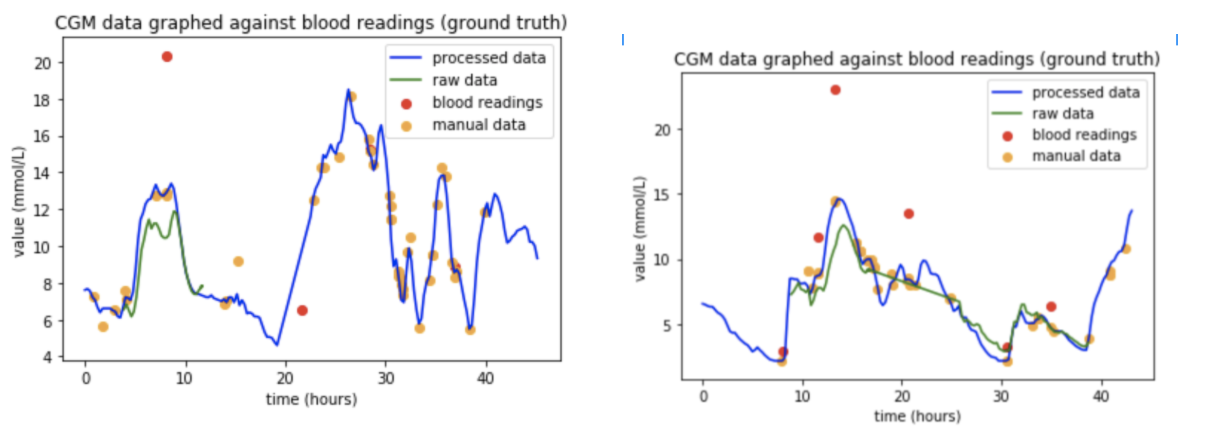
\includegraphics[width=1.0\linewidth]{images/graph0.png}
\caption{Multiple graphs comparing blood glucose data with CGM.}
\label{fig:graph0}
\end{figure}

\section{Prediction}
One of the major additional features that a CGM brings is an element of prediction through data analysis. Improving accuracy of this is very helpful. As previously explained, Freestyle Libre communicates predictions with arrows (see Figure~\ref{fig:arrows}), which translate to the direction glucose is currently trending in mmol/L per minute. First, the accuracy of this needed to be evaluated. The majority of the data we had came in fifteen minute intervals, but it was simple arithmetic to translate the arrow meaning into mmol/L per 15 minute. Matching the time of each manual scan (and hence arrow) to the closest 15 minute change in processed data, an acceptable ground truth, allowed me to get the accuracy of the Freestyle Libre arrows. Depending on the time frame, this varied around 63\% +-5. This seemed fairly low, so effort was made to improve on it using both least squares linear regression and neural networks.

\subsection{Linear Regression}
The initial attempt at linear regression was at seeing whether curve fitting data could be extended to predict future values. As Figure~\ref{fig:graph6} shows, this was predictably unsuccessful. Extending the curve quickly got out of hand, with even the first values being very poorly fit. 

\begin{figure}[ht]
\centering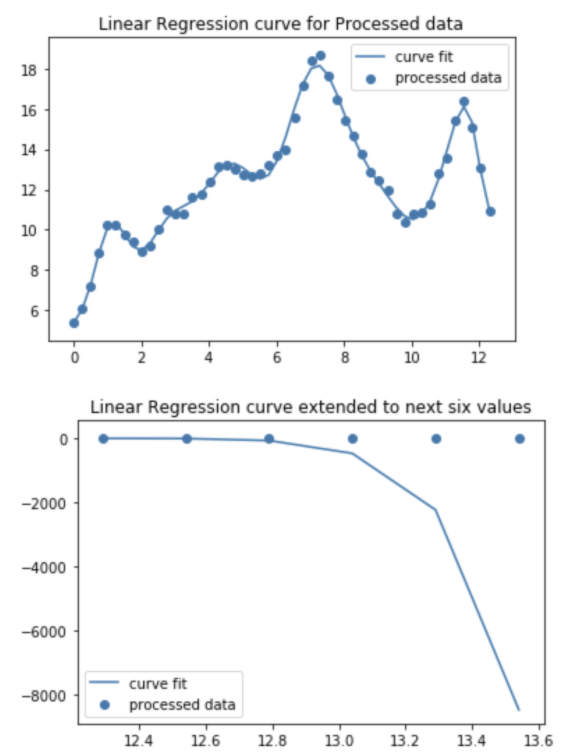
\includegraphics[width=1.0\linewidth]{images/graph6.png}
\caption{Linear Regression results.}
\label{fig:graph6}
\end{figure}

Next, I tried predicting the change in value based on the past 20 datapoints. This initially seemed far more successful than the prior attempt, and even than the reader itself, as shown in Figure~\ref{fig:graph6_5}. The accuracy was taken from testing with separate data, not the training set. While there was some fluctuation depending on the training/test sets chosen, it was consistently above 70\%. Attempting to improve on this - to predict over an hour, to take derivative values as input, to add prior - made little improvement, or caused a backtrack. Nevertheless, it seemed pretty successful.

\begin{figure}[ht]
\centering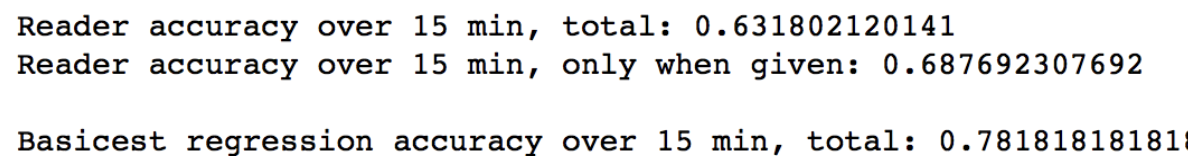
\includegraphics[width=1.0\linewidth]{images/graph6_5.png}
\caption{Linear Regression results on prediction.}
\label{fig:graph6_5}
\end{figure}

\subsection{Neural Networks}
The next attempt at improving on the prediction arrow was a basic neural network, which I expected to be quite successful. However, it would always immediately go to 78\% accuracy and refuse to move through epochs or re-runs, as in Figure~\ref{fig:graph7}. It fluctuated somewhat depending on the testing data, but it was generally settled. This behaviour seemed strange, so I looked further into it.

\begin{figure}[ht]
\centering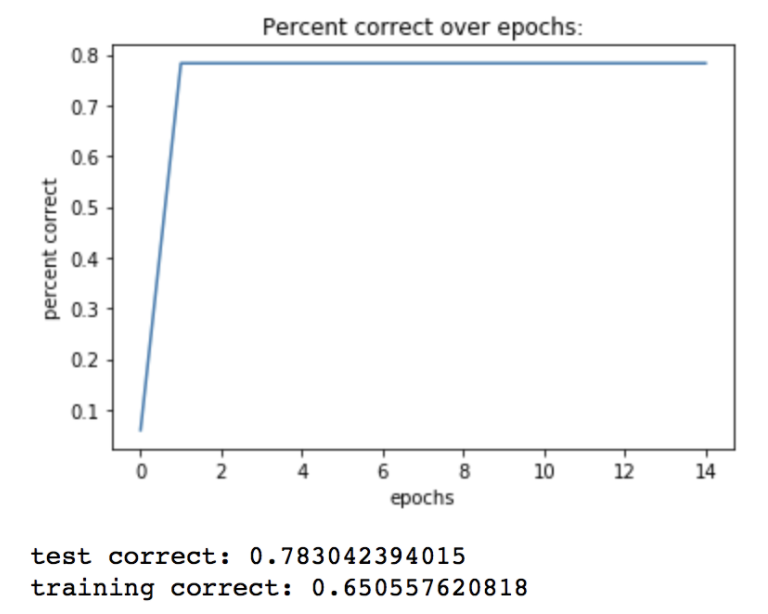
\includegraphics[width=1.0\linewidth]{images/graph7.png}
\caption{Training error against epoch for neural network.}
\label{fig:graph7}
\end{figure}

As it turned out, the problem was that the data was generally too easy to predict. Averaging $\frac{3}{4}$ of it was going straight. This meant the neural network was just persistently returning \textit{straight}, getting it right most of the time, and not changing. In fact, looking back at the linear regression, it suffered the same fault. As Figure~\ref{fig:graph8} shows, the ground truth for the change in value varied between -4 and 4, albeit heavily clustered around zero. The prediction, on the other hand, remains tightly between -1 and 1. This means it still captures most of the data accurately, but ignores two thirds of the possible range.

\begin{figure}[ht]
\centering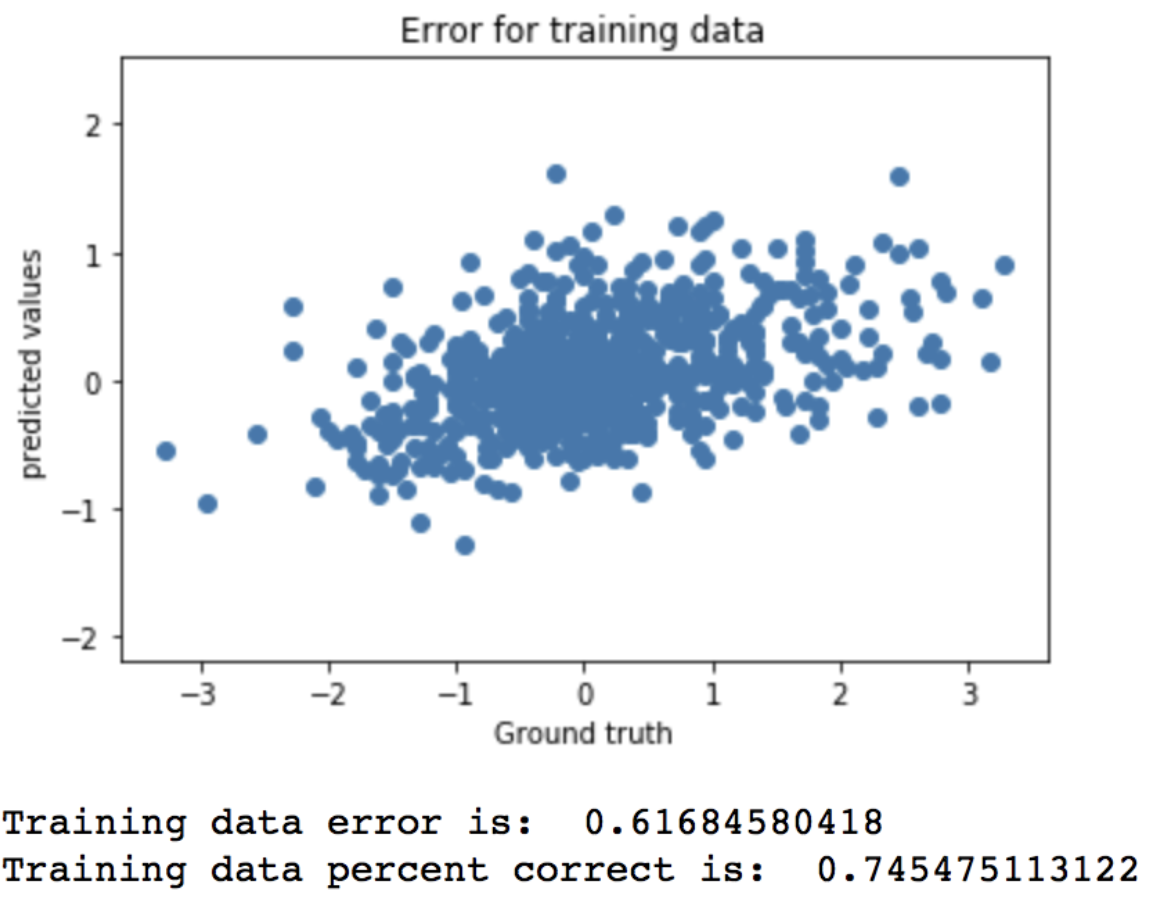
\includegraphics[width=1.0\linewidth]{images/graph8.png}
\caption{Correlation data for prediction.}
\label{fig:graph8}
\end{figure}

\subsection{Reader Prediction Arrow}
The reader’s glucose trend arrow had a poorer mathematical accuracy than either of my algorithms, while displaying the full range of directions instead of just straight. To better understand how this went, I broke down their correct and incorrect instances, as shown in Figure~\ref{fig:graph9}. This shows the distribution of the correct matches, the incorrect arrows, and the incorrectly represented ground truths across the trend directions; the distribution of the differences between a displayed arrow and the corresponding true direction, and a more detailed breakdown of the errors. These numbers tell us a few things.

\begin{figure}[h]
\centering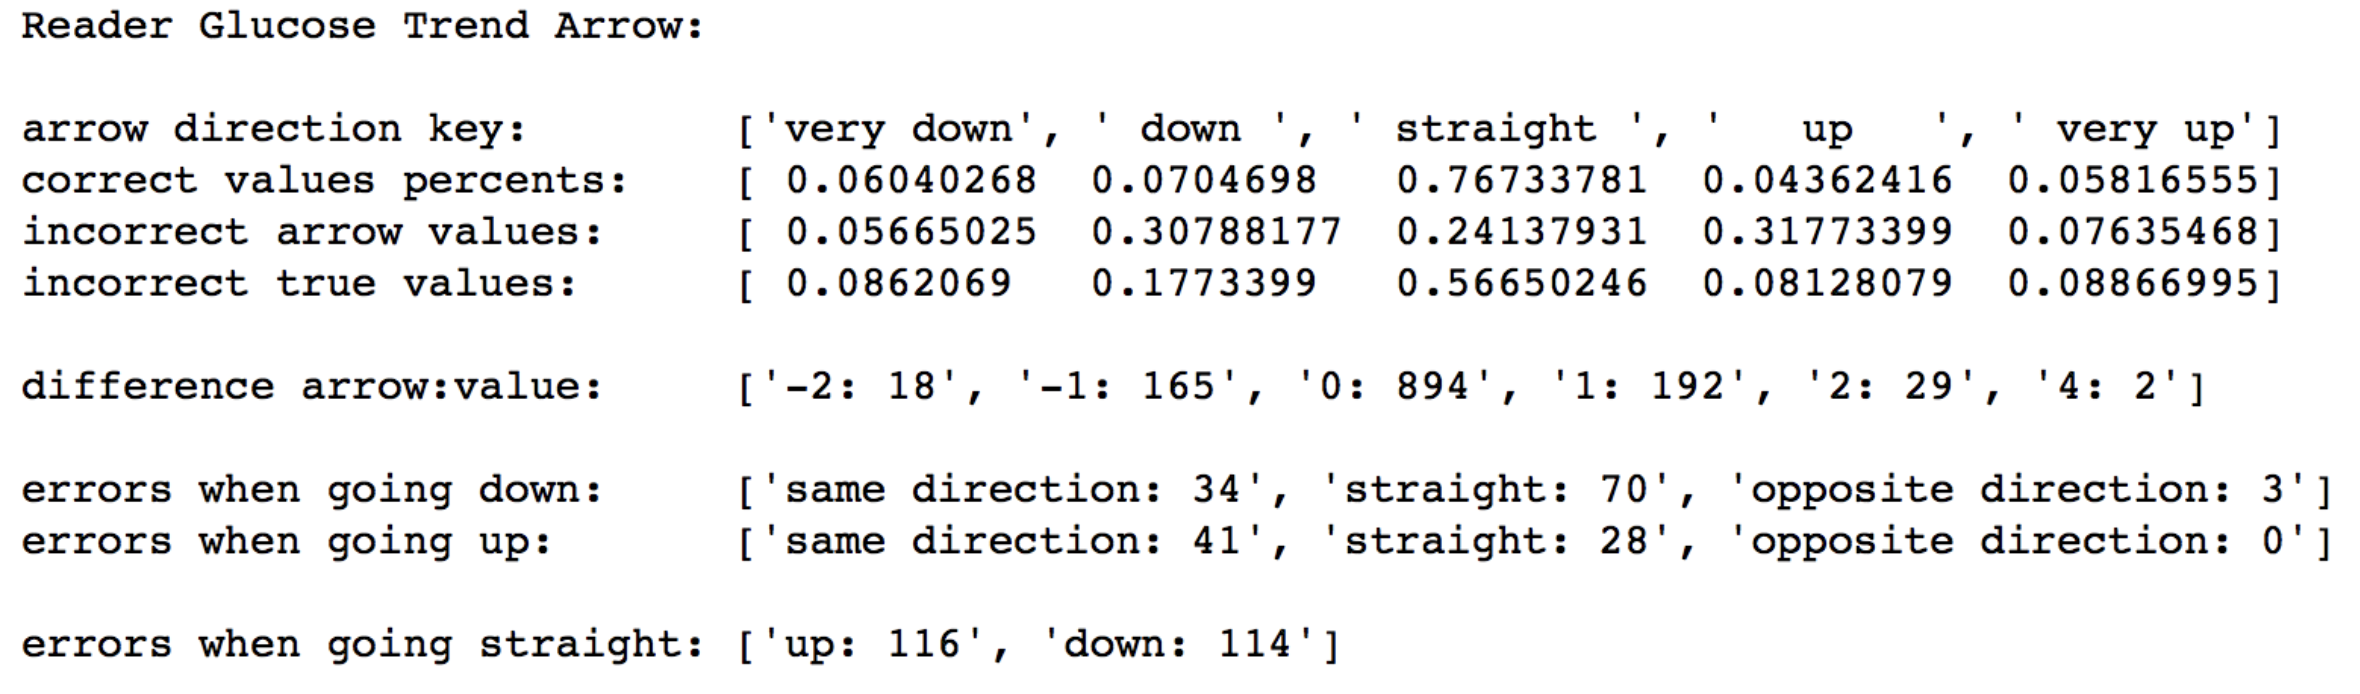
\includegraphics[width=1.0\linewidth]{images/graph9.png}
\caption{Trend arrow statistics.}
\label{fig:graph9}
\end{figure}

First, while the reader is often inaccurate, it’s rarely completely incorrect. Almost 93\% of the predictions is within one degree of the ground truth. Less than 2\% is further away than two degrees. On the other hand, that 2\% is an extreme enough difference to possibly cause harmful management decisions (eg: the difference between 4.2 going straight down, and going straight up). 

The reader exaggerates change. When the reader is correct, it displays a straight arrow 77\% of the time. When the reader is incorrect, it is much more likely to be signalling a change in glucose, only showing straight 24\% of the time. This suggests that the reader algorithm is more responsive to changes in blood glucose than steadiness, and is likely to over exaggerate change in blood glucose. This is in direct contrast to my attempts, which actively conformed everything to ‘straight’, so all the incorrect values were due to rapidly changing bloods being typed as ‘straight’ nonetheless.

On the other hand, the true gradient is more likely to be changing when the reader is incorrect. When the reader was incorrect, the gradient was changing 44\% of the time. This is almost twice the amount when the reader was correct, 23\%. The reader is more likely to read incorrectly on a quickly changing value. Some of this might be overestimating the rate of change, but the rest will be due to underestimating the change. This is in contrast to the early statistics, which suggested that the reader perpetually overestimated change.

With the incorrect readings, the distribution of the true gradient was slightly skewed down. The given arrow value was slightly skewed up. This suggests the reader is more likely to incorrectly predict a higher gradient.

Of the errors that occur while the true value is straight, the uncertainty is very equally distributed between over and underestimating. This suggests a lack of bias. Similarly, the reader has only pointed in completely the wrong direction once. 

When true trend is going down, 60\% of the reader’s incorrect predictions go straight. Only 30\% of the time will an incorrect arrow get the direction, at least, correct. In contrast, if the true trend is up, an incorrect prediction is 60\% likely to be in the right direction, just with the wrong severity. The suggests that the reader arrow exaggerates upwards trends and downplays downwards trends.

The reader’s glucose trend arrow has avoided the trap of only ever predicting straight, while maintaining decent accuracy ratings. It appears to do this by magnifying any change there is in the trend, often resulting in incorrectly predicting more change than there is.


